% !TeX program = pdflatex
% !BIB program = bibtex

\documentclass[12pt,a4paper]{article}
\usepackage{cite}
\usepackage{graphicx}
\usepackage{amsmath}
\usepackage{url}

\graphicspath{ {./assets/} }

\author{Boonyakorn Tanrattanakorn}
\title{Analysis of Transistor-level CMOS Inverter in LTspice}

\begin{document}

\maketitle
\newpage

\section{Design Parameters \& Tool Setup}

\subsection{Parameters}
The NMOS and PMOS transistors are modeled using the typical values for 180nm CMOS Small-Signal Model\cite{mos_parameters}.
The SPICE directives for the NMOS and PMOS transistors are as follows:
\begin{itemize}
    \item \textbf{NMOS:} \texttt{.model NMOS\_180nm NMOS (LEVEL=1 VTO=0.8 KP=90u GAMMA=0.5 PHI=0.68 LAMBDA=0.06)}
    \item \textbf{PMOS:} \texttt{.model PMOS\_180nm PMOS (LEVEL=1 VTO=-0.9 KP=30u GAMMA=0.5 PHI=0.68 LAMBDA=0.06)}
\end{itemize}

\subsection{LTspice Schematic}
\begin{figure}[h]
    \centering
    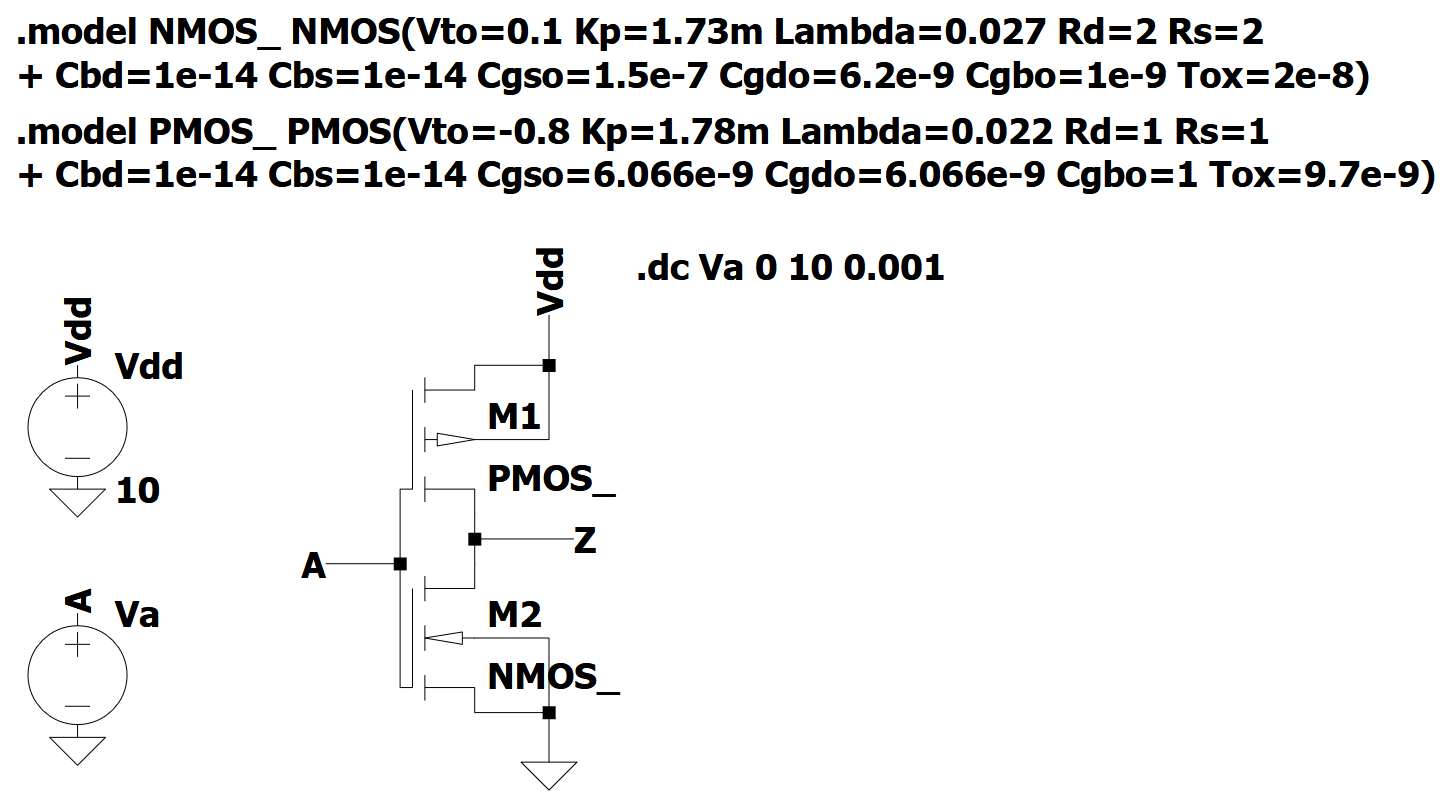
\includegraphics[width=\textwidth]{circuit_setup.png}
    \caption{Circuit setup of the transistor-level CMOS inverter in LTspice.}
    \label{fig:circuit_setup}
\end{figure}

From Fig. \ref{fig:circuit_setup}, the circuit setup of the transistor-level CMOS inverter in LTspice is shown. 
First, on the left side, there are two voltage sources, the power supply voltage (Vdd) is set to 10V
, while V2 represents the input voltage (A). Then, on the
right side, there are two MOSFETs used to represent the PMOS and NMOS transistors. The upper
side is the PMOS transistor, which is connected to Vdd, while the lower side is the NMOS transistor,
which is connected to the ground. Finally, the gate of both transistors is connected to A and
the output voltage (Z) is connected to the junction between the two transistors. 
\cite{mos_parameters}

\section{DC Analysis (Voltage Transfer Characteristics)}
\subsection{VTC Curve Generation}
To obtain the Voltage Transfer Characteristic (VTC), a DC sweep simulation (\texttt{.dc}) is performed, sweeping the input voltage from 0V to [Vdd] with a step size of [Step Size].

\begin{figure}[h]
    \centering
    % 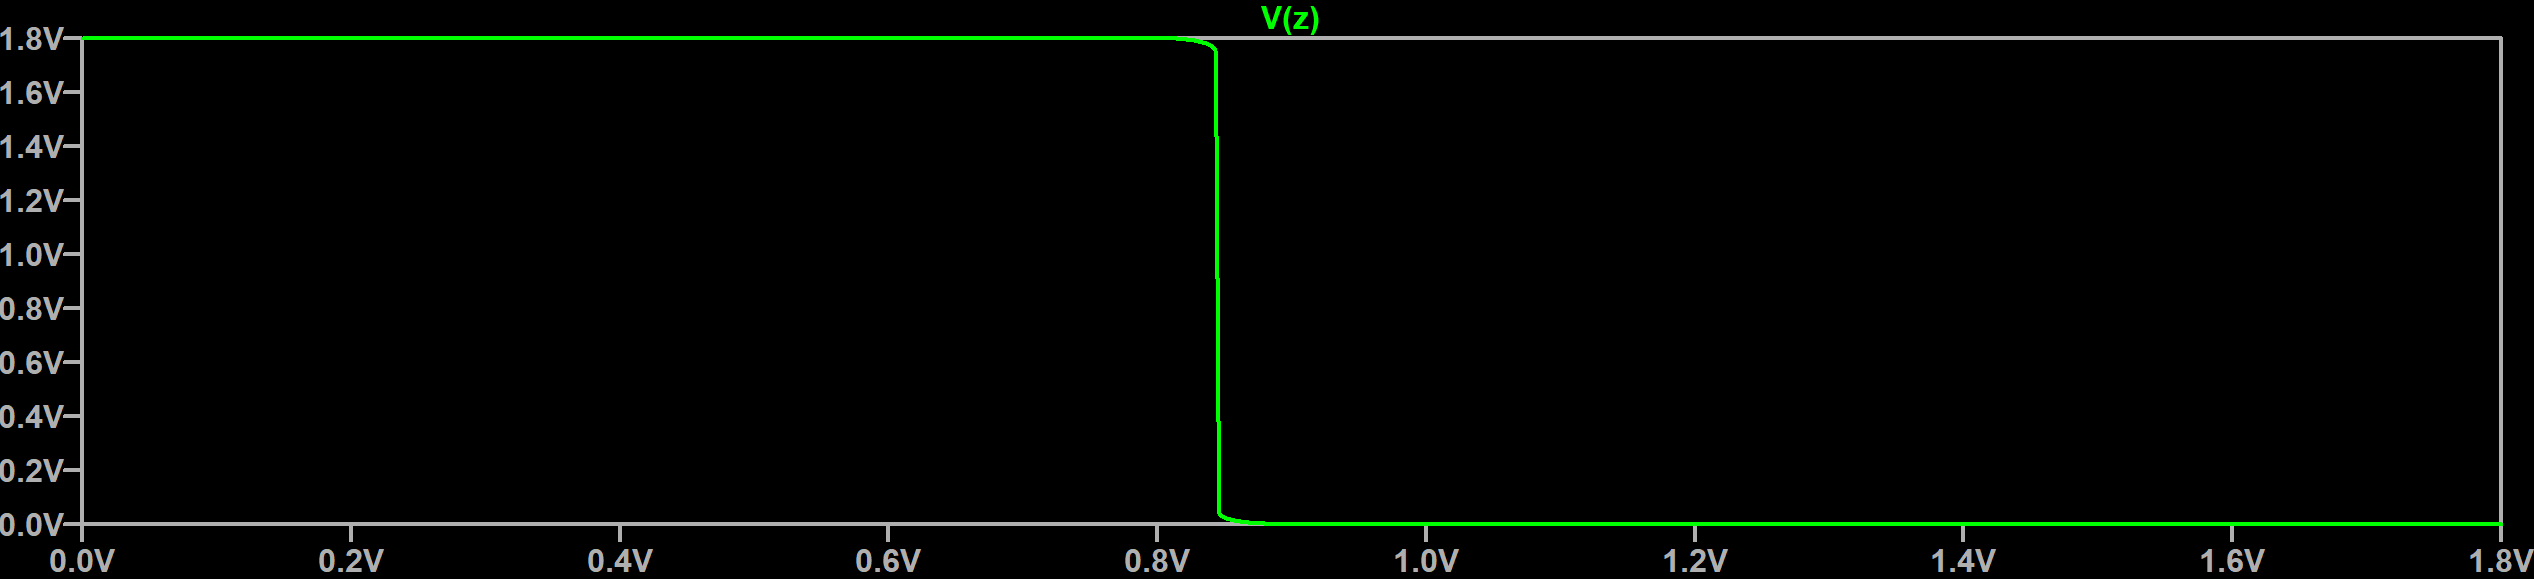
\includegraphics[width=0.8\textwidth]{vtc_curve.png}
    [Insert VTC Curve Graph Here - Uncomment the includegraphics above when ready]
    \caption{Voltage Transfer Characteristic (VTC) of the CMOS Inverter.}
    \label{fig:vtc_curve}
\end{figure}

\subsection{Critical Voltages}
From the VTC curve, the critical voltages are extracted (typically where the slope is -1):
\begin{itemize}
    \item $V_{OH} = $ [Result] V
    \item $V_{OL} = $ [Result] V
    \item $V_{IH} = $ [Result] V
    \item $V_{IL} = $ [Result] V
\end{itemize}

\subsection{Noise Margins}
The noise margins are calculated using the extracted critical voltages:
\begin{itemize}
    \item High Noise Margin ($NM_H = V_{OH} - V_{IH}$) = [Result] V
    \item Low Noise Margin ($NM_L = V_{IL} - V_{OL}$) = [Result] V
\end{itemize}

\subsection{Switching Threshold}
The switching threshold ($V_M$), where $V_{in} = V_{out}$, is measured from the VTC:
\begin{itemize}
    \item $V_M = $ [Result] V
\end{itemize}

\section{Transient Analysis (Timing Characteristics)}
\subsection{Transient Simulation Setup}
To analyze the timing characteristics, a transient simulation (\texttt{.tran}) is performed over [Simulation Time]. The input is driven by a pulse voltage source with the following parameters:
\begin{itemize}
    \item $V_{initial} = $ [0] V, $V_{on} = $ [Vdd] V
    \item $T_{delay} = $ [Delay], $T_{rise} = $ [Rise], $T_{fall} = $ [Fall]
    \item $T_{on} = $ [Pulse Width], $T_{period} = $ [Period]
\end{itemize}

\begin{figure}[h]
    \centering
    % \includegraphics[width=0.8\textwidth]{transient_waveforms.png}
    [Insert Transient Waveforms (Input and Output) Graph Here]
    \caption{Transient response of the CMOS Inverter.}
    \label{fig:transient}
\end{figure}

\subsection{Propagation Delay}
The propagation delay is measured between the 50\% points of the input and output transitions:
\begin{itemize}
    \item High-to-Low Delay ($t_{pHL}$) = [Result]
    \item Low-to-High Delay ($t_{pLH}$) = [Result]
    \item Average Delay ($t_p$) = [Result]
\end{itemize}

\subsection{Rise and Fall Times}
The rise and fall times are measured between the 10\% and 90\% points of the output signal:
\begin{itemize}
    \item Rise Time ($t_r$) = [Result]
    \item Fall Time ($t_f$) = [Result]
\end{itemize}

\section{Power Analysis}
\subsection{Dynamic Power}
Dynamic power dissipation is measured during the transient simulation:
\begin{itemize}
    \item Average Dynamic Power ($P_{dynamic}$) = [Result]
\end{itemize}
% [Optional: Insert plot of instantaneous power/current spikes during transitions here]

\subsection{Static Power}
Static (leakage) power is calculated by measuring the current drawn from Vdd when the inverter state is steady:
\begin{itemize}
    \item Input Low ($V_{in} = 0V$), $P_{static} = $ [Result]
    \item Input High ($V_{in} = Vdd$), $P_{static} = $ [Result]
\end{itemize}

\newpage
\bibliography{references}
\bibliographystyle{plain}

\end{document}